\documentclass[a4paper, 12pt]{article}
\usepackage[a4paper,top=1.5cm, bottom=1.5cm, left=1cm, right=1cm]{geometry}
\usepackage[utf8]{inputenc}
\usepackage{mathtext}
\usepackage{amsmath}
\usepackage{amsfonts}
\usepackage[english, russian]{babel}
\usepackage{indentfirst}
\usepackage{longtable}
\usepackage{graphicx}
\graphicspath{{pictures/}}
\DeclareGraphicsExtensions{.pdf,.png,.jpg}
\usepackage{natbib}
\usepackage{mathrsfs}
%\usepackage[europeanresistors, americaninductors]{circuitikz}

\title{Лабораторная работа 1.2.1 Определение скорости полёта пули при помощи баллистического маятника}
\author{Михаил Колтаков}
\date{9 ноября 2020 г.}

\begin{document}
	\maketitle
	\section*{Цель работы}
		Определить скорость полёта пули применяя законы сохранения и использую баллистические маятники
	\section*{Оборудование}
		Духовое ружьё на штативе, осветитель, оптическая система для измерения отклонений маятника, измерительная линейка, пули и весы для их взвешивания, баллистические маятники.
	\section*{Ход работы}
		\subsection*{I Метод баллистического маятника, совершающего поступательное движение}
			В этой части работы будем использовать установку, изображённую на рисунке ниже. При попадании пули в цилиндр любая его точка движется по окружности известного радиуса, поэтому его смещение с помощью собирающей линзы можно перевести в линейное отклонение на линейке.
			\begin{figure}[h]
				\center{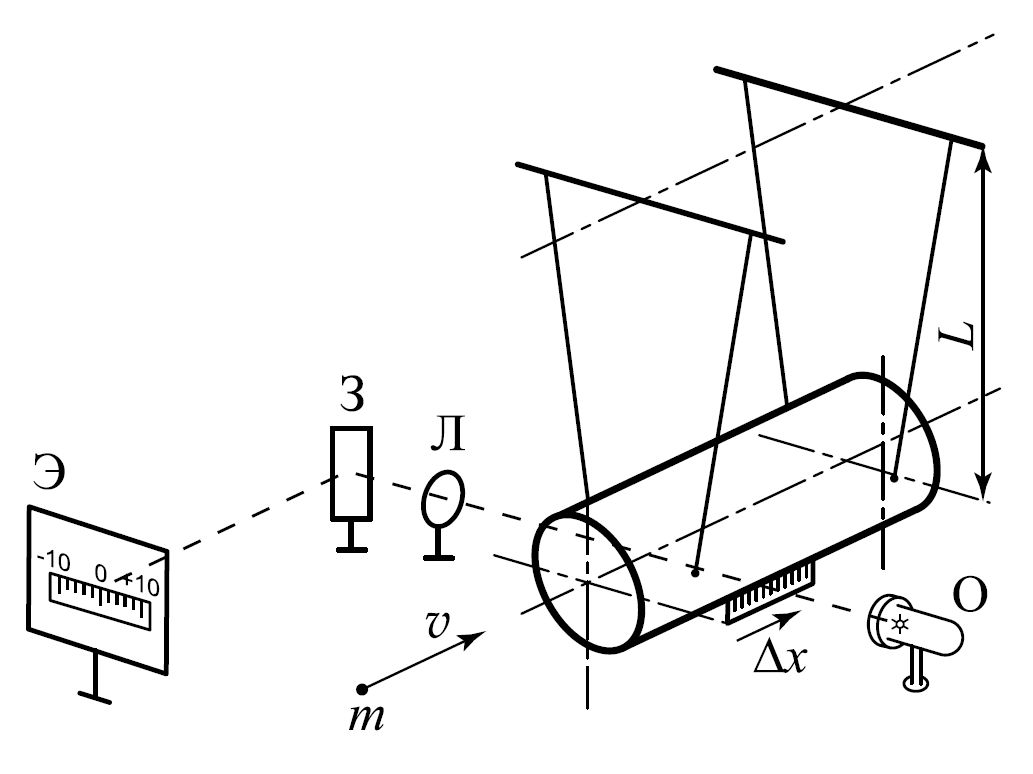
\includegraphics[scale=0.45]{scheme1}}
			\end{figure}
		
			Проверим правильность установки ружья с помощью холостого выстрела. Длина нитей, за которые подвешен цилиндр равна $L \approx 225,5 \pm 1,0 см$. Его масса $M=2905 \pm 5 г$. При контакте пули с цилиндром можно записать ЗСИ
			$$ mu = (M+m)V $$
			$m-масса\: пули$, $u-скорость\: пули\: перед\: ударом$, $V-скорость\: цилиндра\: вместе\: с\: пулей\: после\: удара$.
			$$ u=\frac{M+m}{m}V \approx \frac{M}{m}V \;\;\;\;\;\;\; V^2=2gh \;\;\;\;\;\;\; h = L(1-cos \varphi ) = 2L^2 sin \frac{\varphi^2}{2} \;\;\;\;\;\;\; \varphi \approx \frac{\Delta x}{L} $$
			Тогда скорость пули можно выразить как
			$$ u=\frac{M}{m} \sqrt{\frac{g}{L}} \Delta x $$
			При измерении было замечено, что за 10 периодов амплитуда колебаний почти не уменьшилась, поэтому их затуханием можно пренебречь.
			
			Проведём 4 выстрела и занесём максимальные отклонения, массы пуль и рассчитанную скорость в таблицу
			\begin{longtable}{|c|c|c|c|}
				\hline
				Выстрел & Масса пули, г & $\Delta x$, мм & Скорость пули, м/c\\
				\hline
				1 & 0,503 & 12,8 & 154,2\\
				\hline
				2 & 0,500 & 11,5 & 139,3\\
				\hline
				3 & 0,509 & 12,0 & 142,8\\
				\hline
				4 & 0,506 & 12,0 & 143,6\\
				\hline
			\end{longtable}
			Погрешность измерения таким методом составляет $\Delta u = 10,0 м/с$.
			Среднее значение скорости $\overline{u}=145,0 м/с$, максимальное отклонение от среднего составляет 9,2 м/с
		\subsection*{II Метод крутильного баллистического маятника}
			В этой части работы мы будем использовать крутильный баллистический маятник. Схема установки представлена на картинке ниже.
			\begin{figure}[h]
				\center{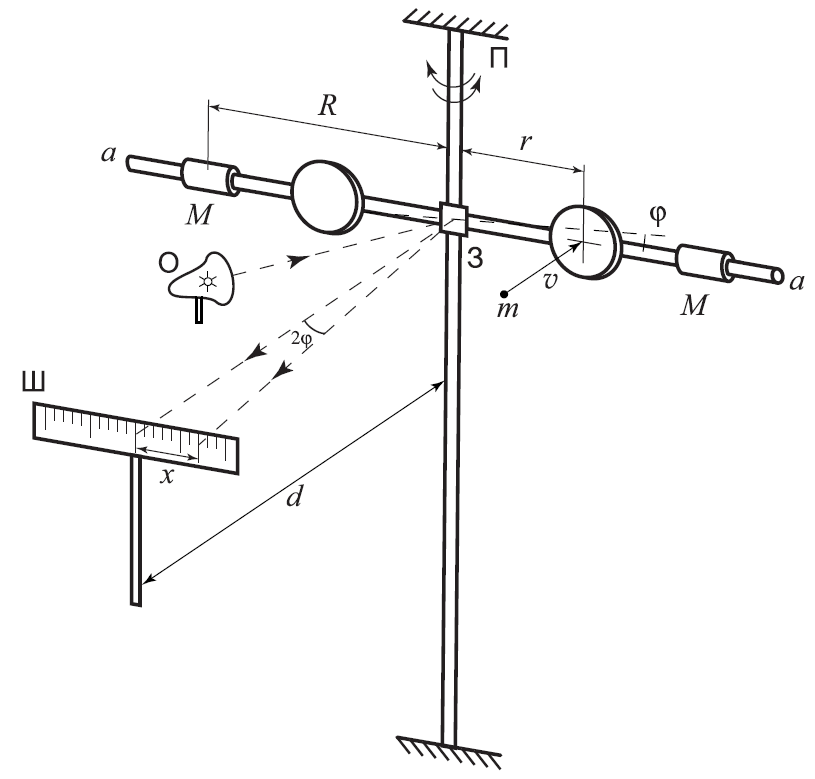
\includegraphics[scale=0.45]{scheme3}}
			\end{figure}
		
			Считая удар неупругим, можно записать уравнение
			$$mur=I \Omega$$
			$r-$расстояние от линии полёта пули до оси вращения, $I$ -- момент инерции относительно этой оси, $\Omega$ -- угловая скорость маятника сразу после удара.
			
			Найдём период колебаний маятника без грузов $T_1 = 9,8 \pm 0,2 с$ и с грузами $T_2 = 13,0 \pm 0,2 с$. Было замечено, что за 10 периодов амплитуда уменьшается меньше, чем в 2 раза. Тогда можно пренебречь затуханием колебаний и потерями энергии и записать ЗСЭ
			$$ k \frac{\varphi^2}{2} = I \frac{\Omega^2}{2} $$
			$k$ -- модуль кручения проволоки, $\varphi$ -- максимальный угол поворота маятника, тогда
			$$ u = \varphi \frac{\sqrt{kI}}{mr} $$
			Измерим растояние от оси вращения до штатива с линейкой $d = 46,0 \pm 0,5 см$, тогда в силу малости колебаний можно найти $\varphi$ как
			$$\varphi \approx \frac{x}{2d}$$
			$x$ -- смещение изображения нити осветителя на шкале, которое легко можно измерить.
			
			Периоды колебаний маятника с грузами и без можно выразить как
			$$T_2 = 2 \pi \sqrt{\frac{I}{k}} \;\;\;\;\;\; T_1= 2 \pi \sqrt{\frac{I - 2MR^2}{k}}$$
			Тогда $\sqrt{kI}$ можно найти как 
			$$\sqrt{kI} = \frac{4 \pi M R^2 T_2}{T_2^2 - T_1^2}$$
			$R = 34,0 \pm 0,5 см$ -- расстояние от оси вращения до центров грузиков, $M = 730,2 г$ - масса грузиков.
			
			Измерим максимальные отклонения маятника, рассчитаем по ним скорость пули и занесём результаты в таблицу.
			\begin{longtable}{|c|c|c|c|c|}
				\hline
				Выстрел & $m$, г & $x$, см & $\varphi$, рад & $u$, м/с \\
				\hline
				1 & 0,505 & 7,8 & 0,085 &  135,0\\
				\hline
				2 & 0,513 & 8,3 & 0,090 &  141,4\\
				\hline
				3 & 0,501 & 7,7 & 0,084 &  134,4\\
				\hline
				4 & 0,513 & 8,0 & 0,087 &  136,3\\
				\hline
			\end{longtable}
		
			Таким образом средняя скорость $\overline{u} = 136,8 м/с$, а максимальное отклонение от неё равно 4,6 м/с. Погрешность измерения скорости таким образом равна $\Delta u \approx 4,7 м/с$
	\section*{Вывод}
		Таким образом, сравнив результаты при использовании двух различных методов определения скорости пули при выстреле из двух идентичных ружей мы получили близкие друг к другу результаты, что означает, что скорее всего, мы определили скорость пули верно. Второй метод, однако, является более точным, так как погрешность экспериментатора, играющая значительную роль при изучении быстрых процессов, в нём значительно меньше.
\end{document}
